\documentclass[usenames,dvipsnames,notes,11pt,aspectratio=169]{beamer}
\usepackage{ifthen}
\usepackage{xcolor}
\usepackage{pgfplots}
\usepackage{amsmath}
\usepackage{centernot}
\usepackage{pifont}
\usepackage{tabularx}
\usepackage{makecell}
\usepackage{cuted}
\usepackage{subcaption}
\usepackage{booktabs}
\usepackage{array}
\usepackage{textcomp}
\usepackage{setspace}
\usepackage{xspace}
\usepackage{tikz}
\usepackage{pdfcomment}
\newcommand{\pdfnote}[1]{\marginnote{\pdfcomment[icon=note]{#1}}}
%\newcommand{\pdfnote}[1]{}

\usepackage{pgfpages}
%\setbeameroption{show notes on second screen}


\input ../beamer-style
\input ../std-macros
\input ../macros

\AtBeginSection[]
{
    \begin{frame}
        \frametitle{Table of Contents}
        \tableofcontents[currentsection]
    \end{frame}
}
\parskip=10pt

\title[CSCI-GA.2590]{Language Models}
\author[He He]{He He
}
\institute[NYU]{New York University}
\date{September 29, 2022}

\begin{document}
\begin{frame}
\titlepage
\end{frame}

\section{Introduction}

\begin{frame}
    {Logistics}
    \begin{itemize}
        \item HW1 due tonight 11:55pm
        \item HW2 released today
    \end{itemize}
\end{frame}

\begin{frame}
    {Last week}
    Goal: Learning useful representions of words

    \textbf{Distributional hypothesis}: Words that occur in similar contexts tend to have similar meanings.

    \begin{spbk}
        {Methods}
    \begin{itemize}
        \item Vector space models: infer clusters from co-occurrence statistics
        \item Self-supervised learning: predict parts of the text (\eg words) from its context (\eg neighbors)
        \item Brown clustering: find word classes in a hierarchical way
    \end{itemize}
    \end{spbk}

    \begin{spbk}
        {Basics of neural networks}
        \begin{itemize}
            \item Learning intermediate subproblems and representations
            \item Activation functions allow for nonlinearity
            \item Optimize by backpropogation (today)
        \end{itemize}
    \end{spbk}
    \pdfnote{
        VSM and BC have disentangled representation in that each coordinate of the word vector has separate meaning.
    }
    \pdfnote{
        SSL is more scalable with large data and flexible in learning objectives.
    }
\end{frame}

\begin{frame}
    {Predict sequences}
    First part:\\
    \begin{itemize}
        \item Text representation $\phi\colon \text{text} \rightarrow \BR^d$
            \begin{itemize}
                \item BoW representation
                \item Distributed representation (word embeddings)
            \end{itemize}
        \item Probabilistic models for classification
            \begin{itemize}
                \item Multinomial Naive Bayes
                \item Logistic regression
            \end{itemize}
    \end{itemize}

    Second part:\\
    \begin{itemize}
        \item Predict sequences
        \item Predict trees
    \end{itemize}

    Today: \blue{probabilistic modeling of sequences}

    \pdfnote{
        Today we'll look at the foundation of sequence prediction,
        language models, which are probabilistic models of word sequences.
        We'll see how we can extend the probabilistic models for a single variable, the class of some input text, to a sequence of variables.
    }
\end{frame}

\begin{frame}
    {Language modeling}
    \beamerblue{Motivation}: pick the most probable sentence from multiple hypothesis
    \begin{itemize}
        \item Speech recognition
            \begin{itemize}
                \item[] the \textit{tail} of a dog
                \item[] the \textit{tale} of a dog
            \end{itemize}
            \begin{itemize}
                \item[] It's not easy to \textit{wreck a nice beach}. 
                \item[] It's not easy to \textit{recognize speech}. 
                \item[] It's not easy to \textit{wreck an ice beach}.
            \end{itemize}
        \item Machine translation 
            \begin{itemize}
                \item[] He sat on the \textit{table}.
                \item[] He sat on the \textit{figure}.
            \end{itemize}
            \begin{itemize}
                \item[] Such a Europe would \textit{the rejection of any} ethnic nationalism. 
                \item[] Such a Europe would \textit{mark the refusal of all} ethnic nationalism. 
            \end{itemize}
    \end{itemize}
    \pdfnote{
        In earlier systems of speech recognition and machine translation,
        the acousitic model and the translation model would produce multiple rough translations, and the language model is used to reweight these outputs by how likely they are English sentences.
    }
\end{frame}

\begin{frame}
    {Language modeling}
    Application: predict/suggest the next word

    \begin{columns}
        \begin{column}{0.5\textwidth}
            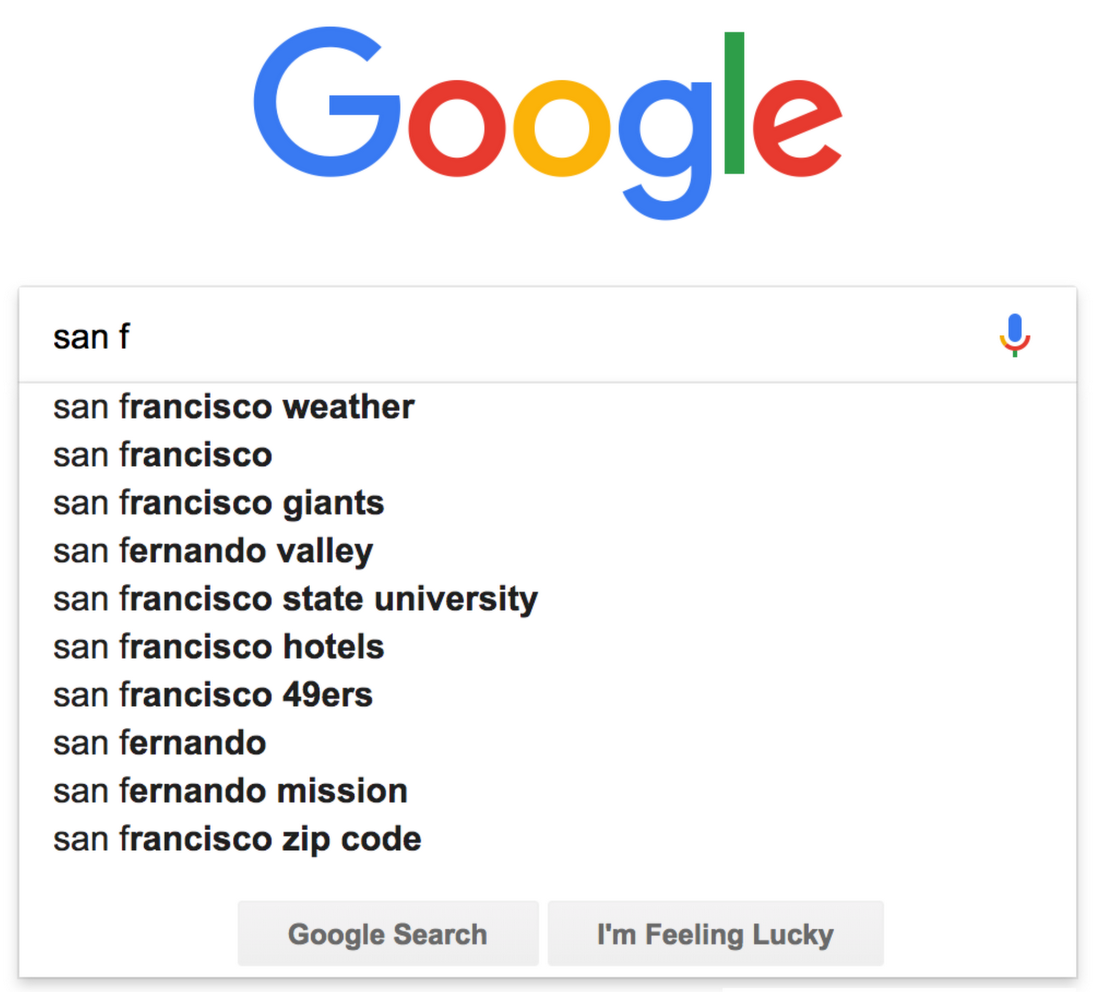
\includegraphics[height=6cm]{figures/autocomplete}
        \end{column}
        \begin{column}{0.5\textwidth}
            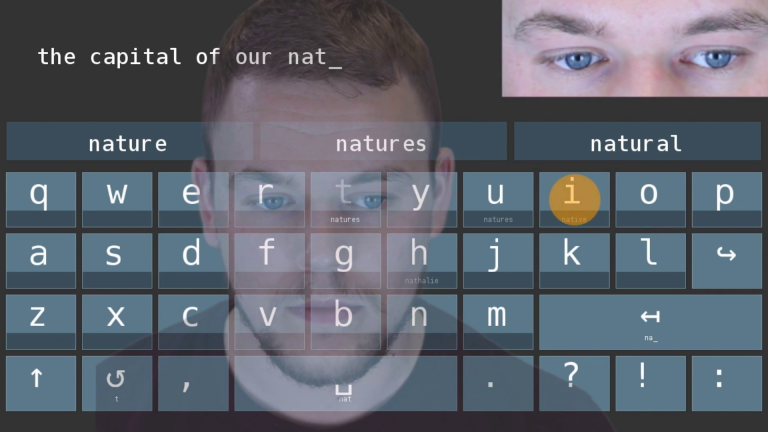
\includegraphics[height=4cm]{figures/gaze}
        \end{column}
    \end{columns}

    \pdfnote{
        When we type our messages, search queries, or emails,
        most interface now provide next word/phrase suggestions to speed up our typing. 
    }
    \pdfnote{
        Another important application is gazed based typing, where people who are physically unable to speak use eye gaze to select words to be spoken by the system.
        This is also applied in VR devices where typing by hand is inconvenient.
    }
\end{frame}

\begin{frame}
    {Problem formulation}
    Assign probabilities to a sequence of tokens:\\
    \begin{itemize}[<+->]
        \item[] $p(\text{the red fox jumped})
            \onslide<+->{\gg} p(\text{the green fox jumped})$
        \item[] $p(\text{colorless green ideas sleep furiously})
            \onslide<+->{\gg} p(\text{furiously sleep ideas green colorless})$
    \end{itemize}

    \begin{itemize}[<+->]
        \item \textbf{Vocabulary}: a \textit{finite} set of symbols $\sV$, e.g.\\
            \indent $\pc{\text{fox}, \text{green}, \text{red}, \text{dreamed}, \text{jumped}, \text{a}, \text{the}}$
        \item \textbf{Sentence}: a \textit{finite} sequence over the vocabulary $x_1 x_2 \ldots x_n \in \sV^n$ where $n\ge 0$ (empty sequence when $n=0$)
        \item The set of all sentences (of different lengths): $\sV^*$ 
        \item Goal: Assign a probability $p(x)$ to all sentences $x\in\sV^*$. 
    \end{itemize}
    \pdfnote{
        red > green: green fox is very rare.
        Grammatically correct sentences is more likely than gibberish.
    }
    \pdfnote{
        Language models tell us how likely we'll encounter a sentence in English. 
        A common misconception is that low probability under an LM means ungrammatical text. However, a sentence can be rare due to many reasons, it could contain rare words, being ungrammatical, or doesn't make any sense. Low probability doesn't necessarily mean ungrammaticality.
    }
    \pdfnote{
        Today, our task is to model this distribution and estimate its params given a corpus.
    }
\end{frame}

\section{N-gram language models}

\begin{frame}
    {Learning a LM}
    \begin{itemize}[<+->]
        \itemsep1em
        \item Given a corpus consisting of a set of sentences: $D=\pc{x^{(i)}}_{i=1}^N$
            \begin{itemize}[<.->]
                \item Notation: $x^{\textstyle\text{(instance id)}}_{\textstyle\text{token id}}$
            \end{itemize}
        \item Consider a multinomial distribution of sentences
            $$
            p_s(x) = \frac{\text{count(x)}}{N} \;.
            $$
            (Exercise: Check that $\sum_{x\in\sV^*}p_s(x) = 1$.)
        \item Is $p_s$ a good LM?
            \begin{itemize}[<+->]
                \item \red{Does not generalize to unseen data.}
                \item Need to restrict the model. 
            \end{itemize}
    \end{itemize}
    \pdfnote{
        Let's consider a multinomial distribution over the sentences,
        where each sentence is an event, and we estimate the probability of each sentence by its fraction in the corpus.
        Specifically, the count of its occurence divided by the total number of sentences.
    }
    \pdfnote{
        This says that our model is too flexible. The number of parameters are the total number of sentences, which increases exponentially with the vocab size. It can approximate any distribution but we won't be able to estimate the model with limited data.
    }
\end{frame}

\begin{frame}
    {Simplification 1: sentence to tokens}
    Solve a smaller problem: model probability of each token

    Decompose the joint probability using the probability \textbf{chain rule}:
            \begin{align*}
                \onslide<+->{
            p(x) &= p(x_1, \ldots, x_n) \\
                &= p(x_1)p(x_2\mid x_1)p(x_3\mid x_1, x_2)\ldots p(x_n\mid x_{1}, \ldots, x_{n-1}) \\
            }
                \onslide<+->{
                & (\text{Doesn't have to go from left to right}) \\
                &= p(x_n)p(x_{n-1}\mid x_n) \ldots p(x_1\mid x_{2},\ldots, x_n)
            }
            \end{align*}

    \begin{itemize}[<+->]
        \item Problem reduced to modeling conditional token probabilities
        %\item Number of outcomes: $|\sV^*|$ (sentences) to $|\sV|$ (symbols)
        \item This is a classification problem we have seen
        \item But there is still a large number of contexts!
    \end{itemize}

\end{frame}

\begin{frame}
    {Simplification 2: limited context}
    Reduce dependence on context by the \textbf{Markov assumption}:\\
    \begin{itemize}
        \item First-order Markov model
            \begin{align*}
                p(x_i\mid x_1,\ldots, x_{i-1}) &= p(x_i\mid x_{i-1}) \\
                p(x) &= \prod_{i=1}^n p(x_i\mid x_{i-1})
            \end{align*}
        \item Number of contexts: $|\sV|$
        \item Number of parameters: \pause $|\sV|^2$
    \end{itemize}

    \pause
    Beginning of a sequence:\\
    $$
    p(x_1\mid x_{1-1}) = ?
    $$
    \pause
    Assume each sequence starts with a special \textbf{start symbol}: $x_0=*$.
\end{frame}

\begin{frame}
    {Model sequences of variable lengths}
    Sample a sequence from the first-order Markov model $p(x_i\mid x_{i-1})$:\\
    \begin{enumerate}
        \item Initial condition: $\text{prev}=\ast$
        \item Iterate:
            \begin{enumerate}
                \item $\text{curr} \sim p(\text{curr}\mid \text{prev})$
                \item $\text{prev}  \leftarrow \text{curr}$
            \end{enumerate}
    \end{enumerate}
    When to stop?

    \pause
    Assume that all sequences end with a \textbf{stop symbol} \texttt{STOP}, e.g.
    \begin{align*}
        &\quad p(\text{the}, \text{fox}, \text{jumped}, \texttt{STOP})\\
         &= p(\text{the}\mid {\color{blue}*})
         p(\text{fox}\mid \text{the})
         p(\text{jumped}\mid \text{fox})
         p({\color{blue}\texttt{STOP}}\mid \text{jumped})
    \end{align*}

    \pause
    LM with the \texttt{STOP} symbol:\\
    \begin{itemize}
        \item Vocabulary: $\texttt{STOP} \in \sV$
        \item Sentence: $x_1 x_2 \ldots x_n \in \sV^n$ for $n\ge 1$ and $x_n=\texttt{STOP}$.
    \end{itemize}
    \pdfnote{
        Accordingly, we'll revise our problem formulation to include the stop symbols.
    }
\end{frame}

\begin{frame}
    {N-gram LM}
    \begin{itemize}
        \item Unigram language model (no context):
            $$
            p(x_1,\ldots, x_n) = \prod_{i=1}^n p(x_i) \;.
            $$
        \item Bigram language model ($x_0=*$):
            $$
            p(x_1,\ldots, x_n) = \prod_{i=1}^n p(x_i\mid x_{i-1}) \;.
            $$
        \item Trigram language model ($x_{-1}=*,x_0=*$):
            $$
            p(x_1,\ldots, x_n) = \prod_{i=1}^n p(x_i\mid x_{i-2}, x_{i-1}) \;.
            $$
        \item $n$-gram language model:
            $$
            p(x_1,\ldots, x_m) = \prod_{i=1}^m p(x_i\mid \underbrace{
                x_{i-n+1},\ldots, x_{i-1}
            }_{\textstyle\text{previous $n-1$ words}} )
            \;.
            $$
    \end{itemize}
\end{frame}

\begin{frame}
    {Practical issues}
    \begin{itemize}
        \itemsep1em
        \item Use $n-1$ start symbols for $n$-gram models
        \item Trigram features are often used in classification
        \item Higher-order models (4/5-grams) are used for MT when large corpus is available
        \item All computation is done in the log space to avoid underflow
    \end{itemize}
\end{frame}

\begin{frame}
    {Parameter estimation}
    \begin{itemize}
        \itemsep1em
        \item Data: a corpus $\pc{x^{(i)}}_{i=1}^N$ where $x\in\sV^n$ denote a sequence.
        \item Model: bigram LM $p(w\mid w')$ for $w,w'\in\sV$.
            $$
            p(w\mid w') = \theta_{w\mid w'} \quad \text{multinomial distribution}
            $$
            where $\sum_{w\in\sV}p(w\mid w') = 1 \quad \forall w'\in\sV$.
    \end{itemize}

    MLE: (HW2 P1)\\
    \gray{[board]} 
\end{frame}

\begin{frame}
    {MLE solution}
    \begin{itemize}
        \itemsep1em
        \item Unigram LM
            $$
            {p}_{\text{MLE}}(x) = \frac{\text{count}(w)}{\sum_{w\in\sV}\text{count}(w)}
            $$
        \item Bigram LM
            $$
            {p}_{\text{MLE}}(w\mid w') =
            \frac{\text{count}(w,w')}{\sum_{w\in\sV}\text{count}(w,w')}
            $$
        \item In general, for n-gram LM,
            $$
            {p}_{\text{MLE}}(w\mid c) =
            \frac{\text{count}(w,c)}{\sum_{w\in\sV}\text{count}(w,c)}
            $$
            where $c\in \sV^{n-1}$.
    \end{itemize}
\end{frame}

\begin{frame}
    {Example}
    \begin{itemize}
        \item Training corpus (after tokenization)
            \begin{itemize}
                \item[] $\pc{\text{The fox is red},
                    \text{The red fox jumped},
                    \text{I saw a red fox}
                    }$
            \end{itemize}
        \item Collect counts
            \begin{itemize}
                \item[] $\text{count}(\text{fox})=3$
                \item[] $\text{count}(\text{red})=3$
                \item[] $\text{count}(\text{red}, \text{fox})=2$
                \item[] $\ldots$
            \end{itemize}
        \item Parameter estimates
            \begin{itemize}
                \item[] $\hat{p}(\text{red}\mid\text{fox})=\pause 2/3$
                \item[] $\hat{p}(\text{saw}\mid\text{i})=\pause 1/1$
            \end{itemize}
        \pause
    \item What is the probability of ``I saw a brown fox jumped''?\pause \hspace{2em} Zero!
    \item What is the probability of ``The fox saw I jumped''?\pause \hspace{2em} Zero!
        \pdfnote{
            Zero probability: OOV words or unseen n-grams.
        }
    \end{itemize}
\end{frame}

\begin{frame}
    {Summary so far}
    \textbf{Language models}: assign probabilities to sentences

    \textbf{N-gram language models}:\\
    \begin{itemize}
        \item Assume each word only conditions on the previous $n-1$ words
        \item MLE estimate: counting n-grams in the training corpus
    \end{itemize}

    Problems with vanilla n-gram models:\\
    \begin{itemize}
        \item Estimate of probabilities involving rare n-grams is inaccurate
        \item Sentences containing unseen n-grams have zero probability
    \end{itemize}
\end{frame}

\begin{frame}
    {Out-of-vocabulary (OOV) words}
    Dealing with OOV words:
    \begin{enumerate}
        \item Choose a fixed vocabulary (\eg all words in the training corpus that occur for more than 5 times)
        \item Replace all OOV words (during training and test) by \texttt{<UNK>}
        \item Treat \texttt{<UNK>} as a normal word
    \end{enumerate}
    \pdfnote{Solving unseen n-grams is harder}
\end{frame}

\begin{frame}
    {Smoothing}
    How to estimate frequencies of unseen words/n-grams?

    More generally, estimate unseen elements in the support of a distribution.\\
    \begin{itemize}
        \item Given frequencies of observed species, what's the probability of encountering a new species?
        \item Given observed genetic variations from a certain population, what's the probability of observing new mutations?
    \end{itemize}

\end{frame}

\begin{frame}
    {Smoothing}
    \beamerblue{Key idea}: reserve some probability mass for unseen words (discounting!)
    \vspace{-1em}
    \begin{figure}
        \begin{subfigure}[b]{\textwidth}
            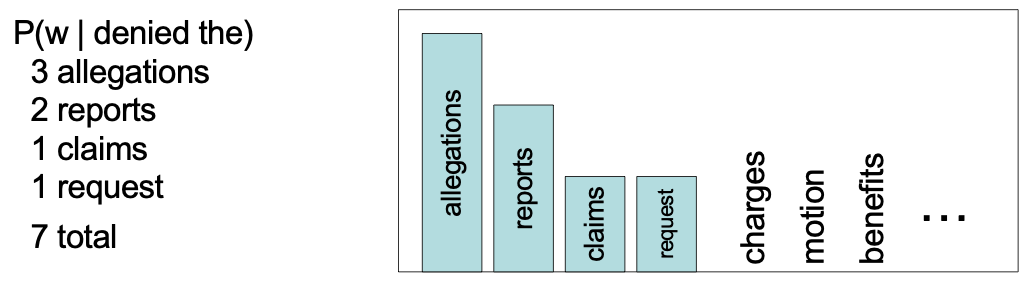
\includegraphics[height=2.5cm]{figures/dist-ori}
        \end{subfigure}\hfill
        \begin{subfigure}[b]{\textwidth}
            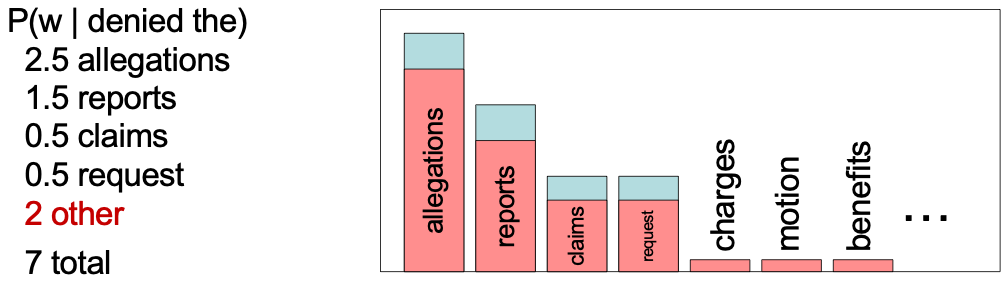
\includegraphics[height=2.5cm]{figures/dist-disc}
        \end{subfigure}
    \end{figure}
    (Figures from Dan Klein and John DeNero)
\end{frame}

\begin{frame}
    {Add-$\alpha$ smoothing}
    Original estimate: \\
    $$
    \frac{\text{count}(x)}{N}
    $$
    \pause

    Smoothed estiamte (add \blue{pseudo count} to each word):\\ 
    $$
    \frac{\text{count}(x) + \mblue{\alpha}}{N + \mblue{\alpha |\sV|}}
    $$
    \pause

    Discounted counts:\\
    \begin{align}
        \frac{\text{count}^*(x)}{N} &= 
\frac{\text{count}(x) + {\alpha}}{N + {\alpha |\sV|}}\\
        \text{count}^*(x) &= \frac{N}{N + {\alpha |\sV|}} (\text{count}(x) + \alpha)
    \end{align}
\end{frame}

\begin{frame}
    {Add-one smoothing}
    How does smoothing change the estimate?

    Example:\\
    \begin{itemize}
        \item[] $\text{count}(x)=10, N=100, |\sV|=1000$
        \item[] Original: $10/100=0.1$
        \item[] Smoothed: $(10+1)/(100+1000)\approx 0.01$
    \end{itemize}

    \pause
    Assigns too much probability mass to unseen words!

    Tuning $\alpha$ on validation set helps but still not good enough for LM in practice.
\end{frame}

\begin{frame}
    {Good-Turing smoothing}
    \beamerblue{Key idea}: use a held-out (validation) set to estimate the ``correct'' counts and adjust the raw count accordingly\\

    Leave-one-out cross validation\\

    \gray{[board]}

\end{frame}

\begin{frame}
    {Good-Turing smoothing}
    \begin{itemize}
        \item Let $M$ be the total number of tokens
        \item Let $N_r$ be the number of word types that occur $r$ times in the corpus
            \pause
            \pdfnote{difference between type and token}
        \item How many held-out tokens are unseen during training? 
            \pause$N_1$
        \item How many held-out tokens are seen $k$ times during training? 
            \pause$N_{k+1}(k+1)$
            \pdfnote{
                Note that there are N k+1 types that occur k times during training and once in validation.
                The number of tokens will be number of types multiplied by k+1.
            }
        \pause
        \item What's the ``correct'' count of a word that occur $k$ times in the corpus?
            $$
            N_k\text{count}^*(x) = N_{k+1}(k+1)
            $$
            \pdfnote{
                There are N k such words, each occuring x times in the training.
                The total counts should be equal to the gold counts in the held-out set.
            }
            \pause
        \item What's the probability of a word that occur $k$ times in training?
            \begin{align*}
                \hat{p}_k(x) &= \frac{\text{count}^*(x)}{M} = \frac{(k+1)N_{k+1}}{MN_k}\\
                \hat{p}_0 &= \frac{N_1}{M}
            \end{align*}
    \end{itemize}
\end{frame}


\begin{frame}
    {Backoff}
    \pdfnote{Backoff and interpolation are often used together with smoothing.
    }
    \beamerblue{Problem}: Cannot estiamte probability of rare $n$-grams accurately

    \beamerblue{Idea}:
    Use higher-order models when we have enough evidence.

    \pdfnote{
        We cannot estimate probs of rare n-grams accurately.
        An n-gram becomes more infrequrent as n increases.
        But if we set n to be too small it may be model dependencies among words that's needed for our task.
        So the idea here is that let's choose the context size dynamically and only use longer context when we have enough evidence.
        For example, if we have observed the trigram ``dark brown fox'' many times, use the MLE estimate, otherwise use the estimate of ``brown fox'', so on and so forth.
    }

    \pause
    {First try}:
    $$
    {p}_{\text{backoff}}(x_i\mid x_{i-n+1:i-1}) =  
    \begin{cases}
        p_{\text{MLE}}(\mred{x_i\mid x_{i-n+1:i-1}}) & \text{if } \text{count}(x_{i-n+1:i}) > 0 \\
        \mblue{\alpha} {p}_{\text{backoff}}(\mgreen{x_i\mid x_{i-n+2:i-1}}) & \text{otherwise}
    \end{cases}
        %\frac{\text{count}(x_{i-n+1:i})}{\text{count}(x_{i-n+1:i-1})} & \text{if } \text{count}(x_{i-n+1:i}) > 0 \\
    $$
    \begin{itemize}
        \item If the \red{$n$-gram} has occured in the corpus, use the MLE estimate
        \item Otherwise, backoff to the \green{$n-1$ gram} estimate recursively with a \blue{constant backoff factor}
            \pause
        \item Not a proper probability distribution because of additional probability mass on unseen $n$-grams
        \item But works well in practice (Stupid Backoff \mycite{[Brants et al., 2007]})
    \end{itemize}
\end{frame}

\begin{frame}
    {Backoff}
    \beamerblue{Problem}: Cannot estiamte probability of rare $n$-grams accurately

    \beamerblue{Idea}:
    Use higher-order models when we have enough evidence.

    {Second try (Katz Backoff)}:
    $$
    {p}_{\text{backoff}}(x_i\mid x_{i-n+1:i-1}) =  
    \begin{cases}
        \mblue{p_{\text{discount}}}({x_i\mid x_{i-n+1:i-1}}) & \text{if } \text{count}(x_{i-n+1:i}) > 0 \\
        \mred{\alpha(x_{i-n+1:i-1})} {p}_{\text{backoff}}({x_i\mid x_{i-n+2:i-1}}) & \text{otherwise}
    \end{cases}
        %\frac{\text{count}(x_{i-n+1:i})}{\text{count}(x_{i-n+1:i-1})} & \text{if } \text{count}(x_{i-n+1:i}) > 0 \\
    $$

    \begin{itemize}
        \item \blue{Discounted probability}: reserve some probability mass for unseen events%, \eg subtracting counts
        \item  \red{Backoff factor}: probability mass distributed to unseen events given a specific context
    \end{itemize}
    \pdfnote{Discounting is a recurring idea in n-gram LM.}
\end{frame}

\begin{frame}
    {Interpolation}
    Instead of backing off to lower-order models, we can use a  \blue{mixture of n-gram models}
    $$
    p(x_i\mid x_{i-2}, x_{i-1}) = \lambda_1 p(x_i\mid x_{i-2}, x_{i-1})
    + \lambda_2 p(x_i\mid x_{i-1})
    + \lambda_3 p(x_i)
    $$
    where $\lambda_1 + \lambda_2 + \lambda_3=1$ (why?).
    \pdfnote{Make sure it's a valid prob dist.}

    \begin{itemize}
        \item $\lambda$ can depend on context: $\lambda(x_{i-2}, x_{i-1})$.
        \item Tune $\lambda$'s on the validation set.
        \item Model $\lambda$ as a latent variable and solve by EM algorithm (later)
            \pdfnote{
                Before generating each word, we first choose a latent context size, then generate according to the corresponding n-gram model.
            }
    \end{itemize}
\end{frame}

\begin{frame}
    {Kneser-Ney smoothing}
    \pdfnote{KN smoothing is the most widely used n-gram LMs that combines multiple ideas we have seen.}
    Widely used for n-gram LMs.

    \beamerblue{Idea 1}: absolute discounting.
    \begin{figure}
        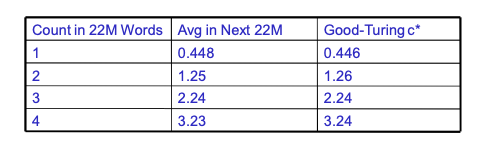
\includegraphics[height=3cm]{figures/good-turing}
        \caption{Good-Turing counts from Dan Klein's slides}
    \end{figure}

    Just subtract 0.75 or some constant.
\end{frame}

\begin{frame}
    {Kneser-Ney smoothing}
    \beamerblue{Idea 2}: consider word \blue{versatility} rather than word counts.

    \beamerblue{Motivation}:\\
    \begin{itemize}
        \item[] $\text{count}(\text{Francisco})=100$, $\text{count}(\text{Minneapolis})=10$
        \item[] I recently visited $\rule{1cm}{0.15mm}$.
    \end{itemize}
    \pdfnote{Which one is more likeley? While Francisco occurs more frequently, it only following the word ``San''.}
    \pause
    Some words can only follow specific contexts, i.e. less versatile.

    \textbf{Continuation probability}: how likely is $w$ allowed in a context $c$\\
        %\item[] $p_{\text{unigram}}(w) \propto \sum_{w'\in\sV}\text{count}(w, w')$
            \begin{align*}
                p_{\text{continuation}}(w) &\propto |\pc{w'\colon \text{count}(w', w) > 0}| \quad \text{\# of context $w$ can follow}\\
                &= \frac{|\pc{w'\colon \text{count}(w', w) > 0}|} 
                {\sum_{w}|\pc{w'\colon \text{count}(w', w) > 0}|} \\
                &= \frac{\text{\# bigram types ends with $w$}}{\text{\# bigram types}}
            \end{align*}
\end{frame}

\begin{frame}
    {Kneser-Ney smoothing}
    Combine the two ideas: \blue{absolute discount} and \green{continuation probability}

    For bigrams:\vspace{-1em}
    $$
    {p}_{KN}(w\mid w') = \frac{\max(\text{count}(w, w') \mblue{- d}, 0)}{\text{count(w')}} + \red{\lambda(w')}\mgreen{p_{\text{continuation}}}(w)
    $$

    \begin{itemize}
        \item \red{$\lambda$}: discounted probability mass
        \item Works well for ASR and MT.
        \item Dominating n-gram model before neural LMs.
    \end{itemize}
\end{frame}

\begin{frame}
    {Real n-gram counts}
    Google Books n-gram counts
    \begin{figure}
        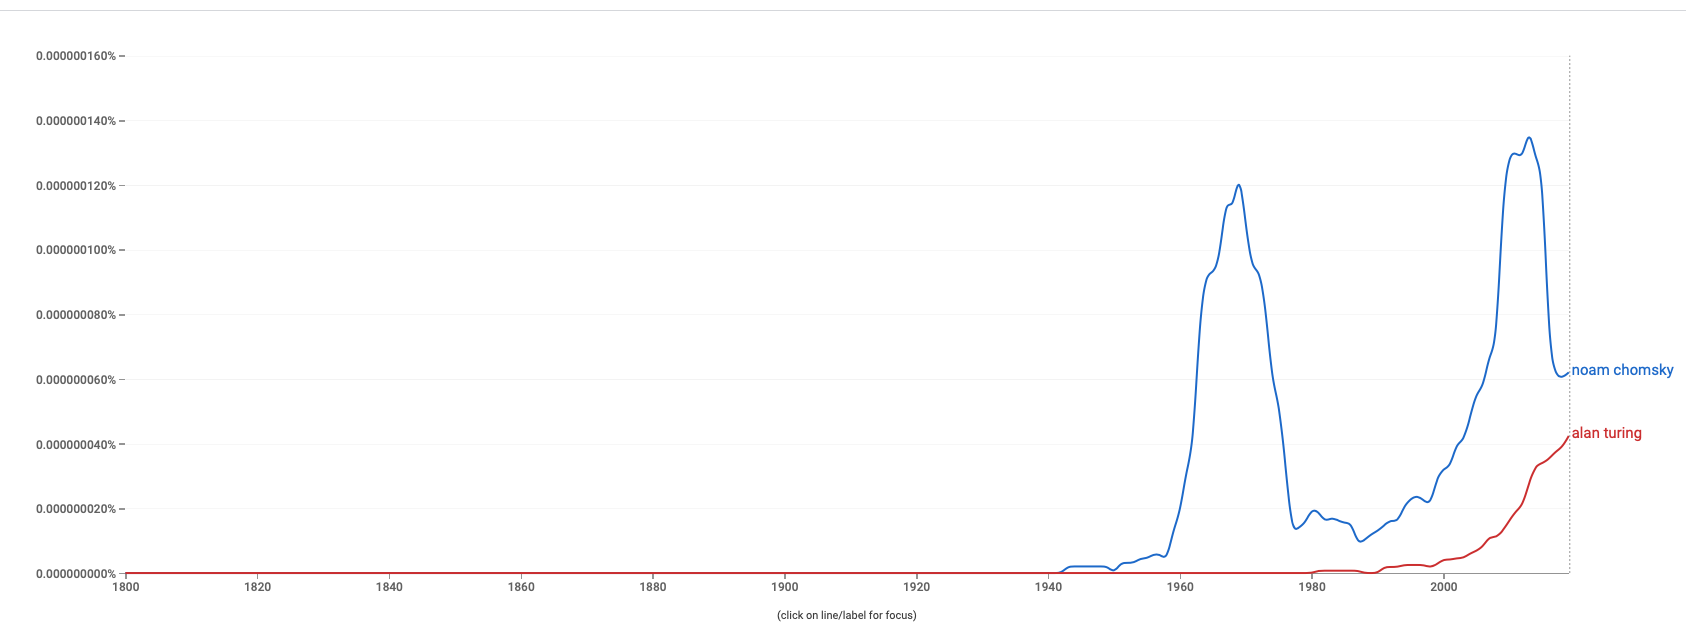
\includegraphics[height=3cm]{figures/google-ngram}
    \end{figure}

    Efficient implementation\\
    \begin{itemize}
        \item Memory, inference speed
            \pdfnote{Large number of n-grams to save!}
        \item Context encodings, tries, caching, ...
            \pdfnote{Definitely don't want to save the strings. Lots of research work on making it efficient.}
        \item \texttt{kenlm} (\url{https://github.com/kpu/kenlm})
            \pdfnote{A fast n-gram model if you ever need one.}
    \end{itemize}
\end{frame}


\begin{frame}
    {Summary}
    Key ideas in n-gram language models to handle sparsity:

    \textbf{Markov assumption}:\\
    \begin{itemize}
        \item Trigram models are reasonable.
        \item ASR, MT often use 4- or 5-gram models.
    \end{itemize}

    \textbf{Discounting / Smoothing}:\\
    \begin{itemize}
        \item ``Borrow'' probability mass for unseen words
        \item Good-Turing smoothing, absolute discount
    \end{itemize}

    \textbf{Dynamic context}:\\
    \begin{itemize}
        \item Use more context if there is evidence
        \item Katz backoff, Kneser-Ney
    \end{itemize}

    See Chen and Goodman (1999) for more results.
\end{frame}

\section{Neural language models}
\begin{frame}
    {N-gram models by classification}
    \pdfnote{In the previous section, we fit a multinomial distribution for the words in each context. Let's now see how we can formulate word prediction as a classification problem.}
    \textbf{Log-linear} language model:
    $$
    p(w\mid c) = \frac{
        \exp\pb{\theta\cdot \phi(w, c)}
    }{
        \sum_{w'\in\sV}\exp\pb{\theta\cdot \phi(w', c)}
    }
    $$
    \begin{itemize}
        \item Predict the output word given the context, \eg $c=\text{the brown fox}$ and $w=\text{jumped}$
        \item Use compatibility scores: $\theta_w\cdot\phi(c) \rightarrow  \theta\cdot\phi(w, c)$ 
    \end{itemize}
\end{frame}

\begin{frame}
    {N-gram models by classification}
    How to design the feature map $\phi(w, c)$?

    Corpus: ``the brown fox jumped''
    \pause

    \pdfnote{Using compatibility scoers, we can design features by characterizing a word and its context}
    \begin{enumerate}
        \item Define feature templates:
            \begin{itemize}
                \item[] $T_1(w,c)=(w, c[-1])$ (bigram feature)
                \item[] $T_2(w,c)=(w, \text{POS}(c[-1]))$
                \item[] $T_3(w,c)=(w, \text{suffix}(c[-1]))$
            \end{itemize}
            \pause
    \item Read off features from the data
        \begin{itemize}
            \item[] $\phi_1(w, c) = \mathbb{I}(w=\text{the}, c[-1]=*)$
            \item[] $\phi_2(w, c) = \mathbb{I}(w=\text{brown}, c[-1]=\text{the})$
        \end{itemize}
    \end{enumerate}
    \begin{itemize}
        \item Each template can produce many features
        \item Each class (word) has different features
            \pdfnote{Note that if brown has never occured at the beginning of the sentence in our corpus, then we won't have the bigram feature *brown.}
    \end{itemize}
\end{frame}

\begin{frame}
    {Feed-forward neural networks}
    Key idea in neural nets: feature/representation learning 

    Building blocks:\\
    \begin{itemize}
        \itemsep2em
        \item Input layer: raw features (no learnable parameters)
        \item Hidden layer: perceptron + nonlinear activation function
        \item Output layer: linear (+ transformation, e.g. softmax)
    \end{itemize}
\end{frame}

\begin{frame}
    {Feed-forward neural language models}
    Encode the \emph{fixed-length} context using feed-forward NN:
    \pdfnote{talk about each layer}
    \begin{figure}
        \includegraphics[height=5cm]{figures/fflm}
    \end{figure}
    What kind of features may be learned?
    \pdfnote{
        Word embedding can encode any feature about a single words, e.g. prefix/suffix, POS tags etc.
        The merge step allows for interaction among words in the context, e.g. bigram.
    }
\end{frame}

\begin{frame}
{Computation graphs}
Function as a \emph{node} that takes in \emph{inputs} and produces \emph{outputs}.

\begin{columns}[t]
\column{.5\textwidth}
\begin{itemize}
\item Typical computation graph:
\end{itemize}
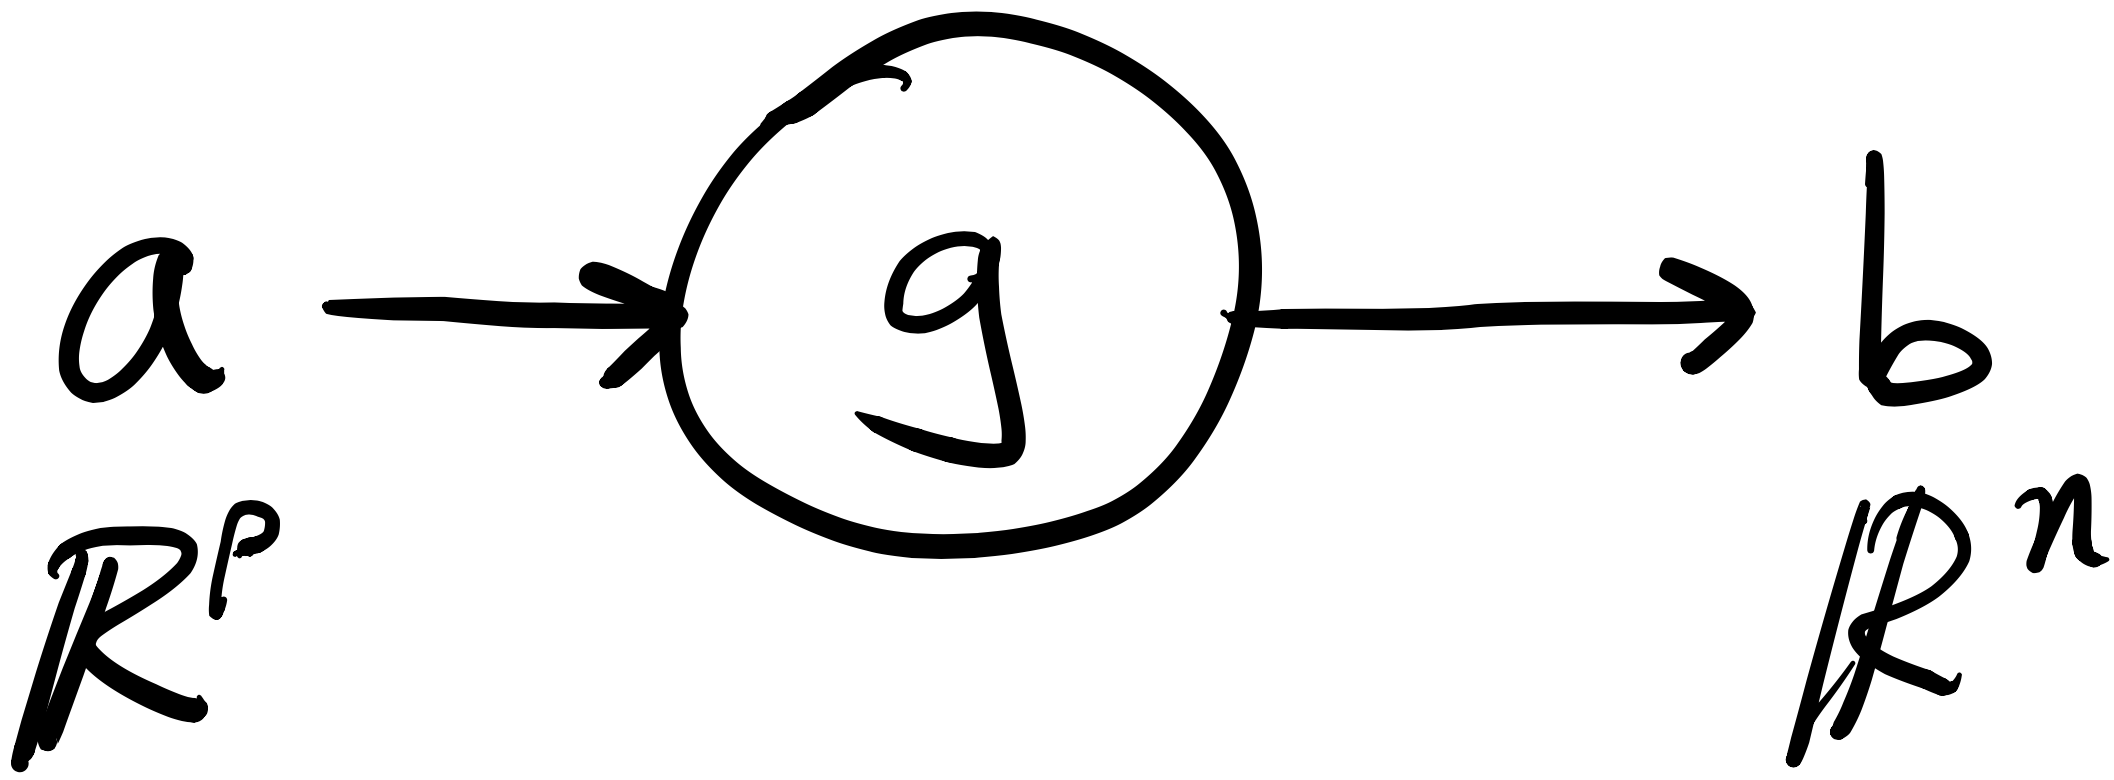
\includegraphics[scale=0.05]{figures/one-fn-comp-graph}

\column{.5\textwidth}
\begin{itemize}
\item Broken out into components:
\end{itemize}
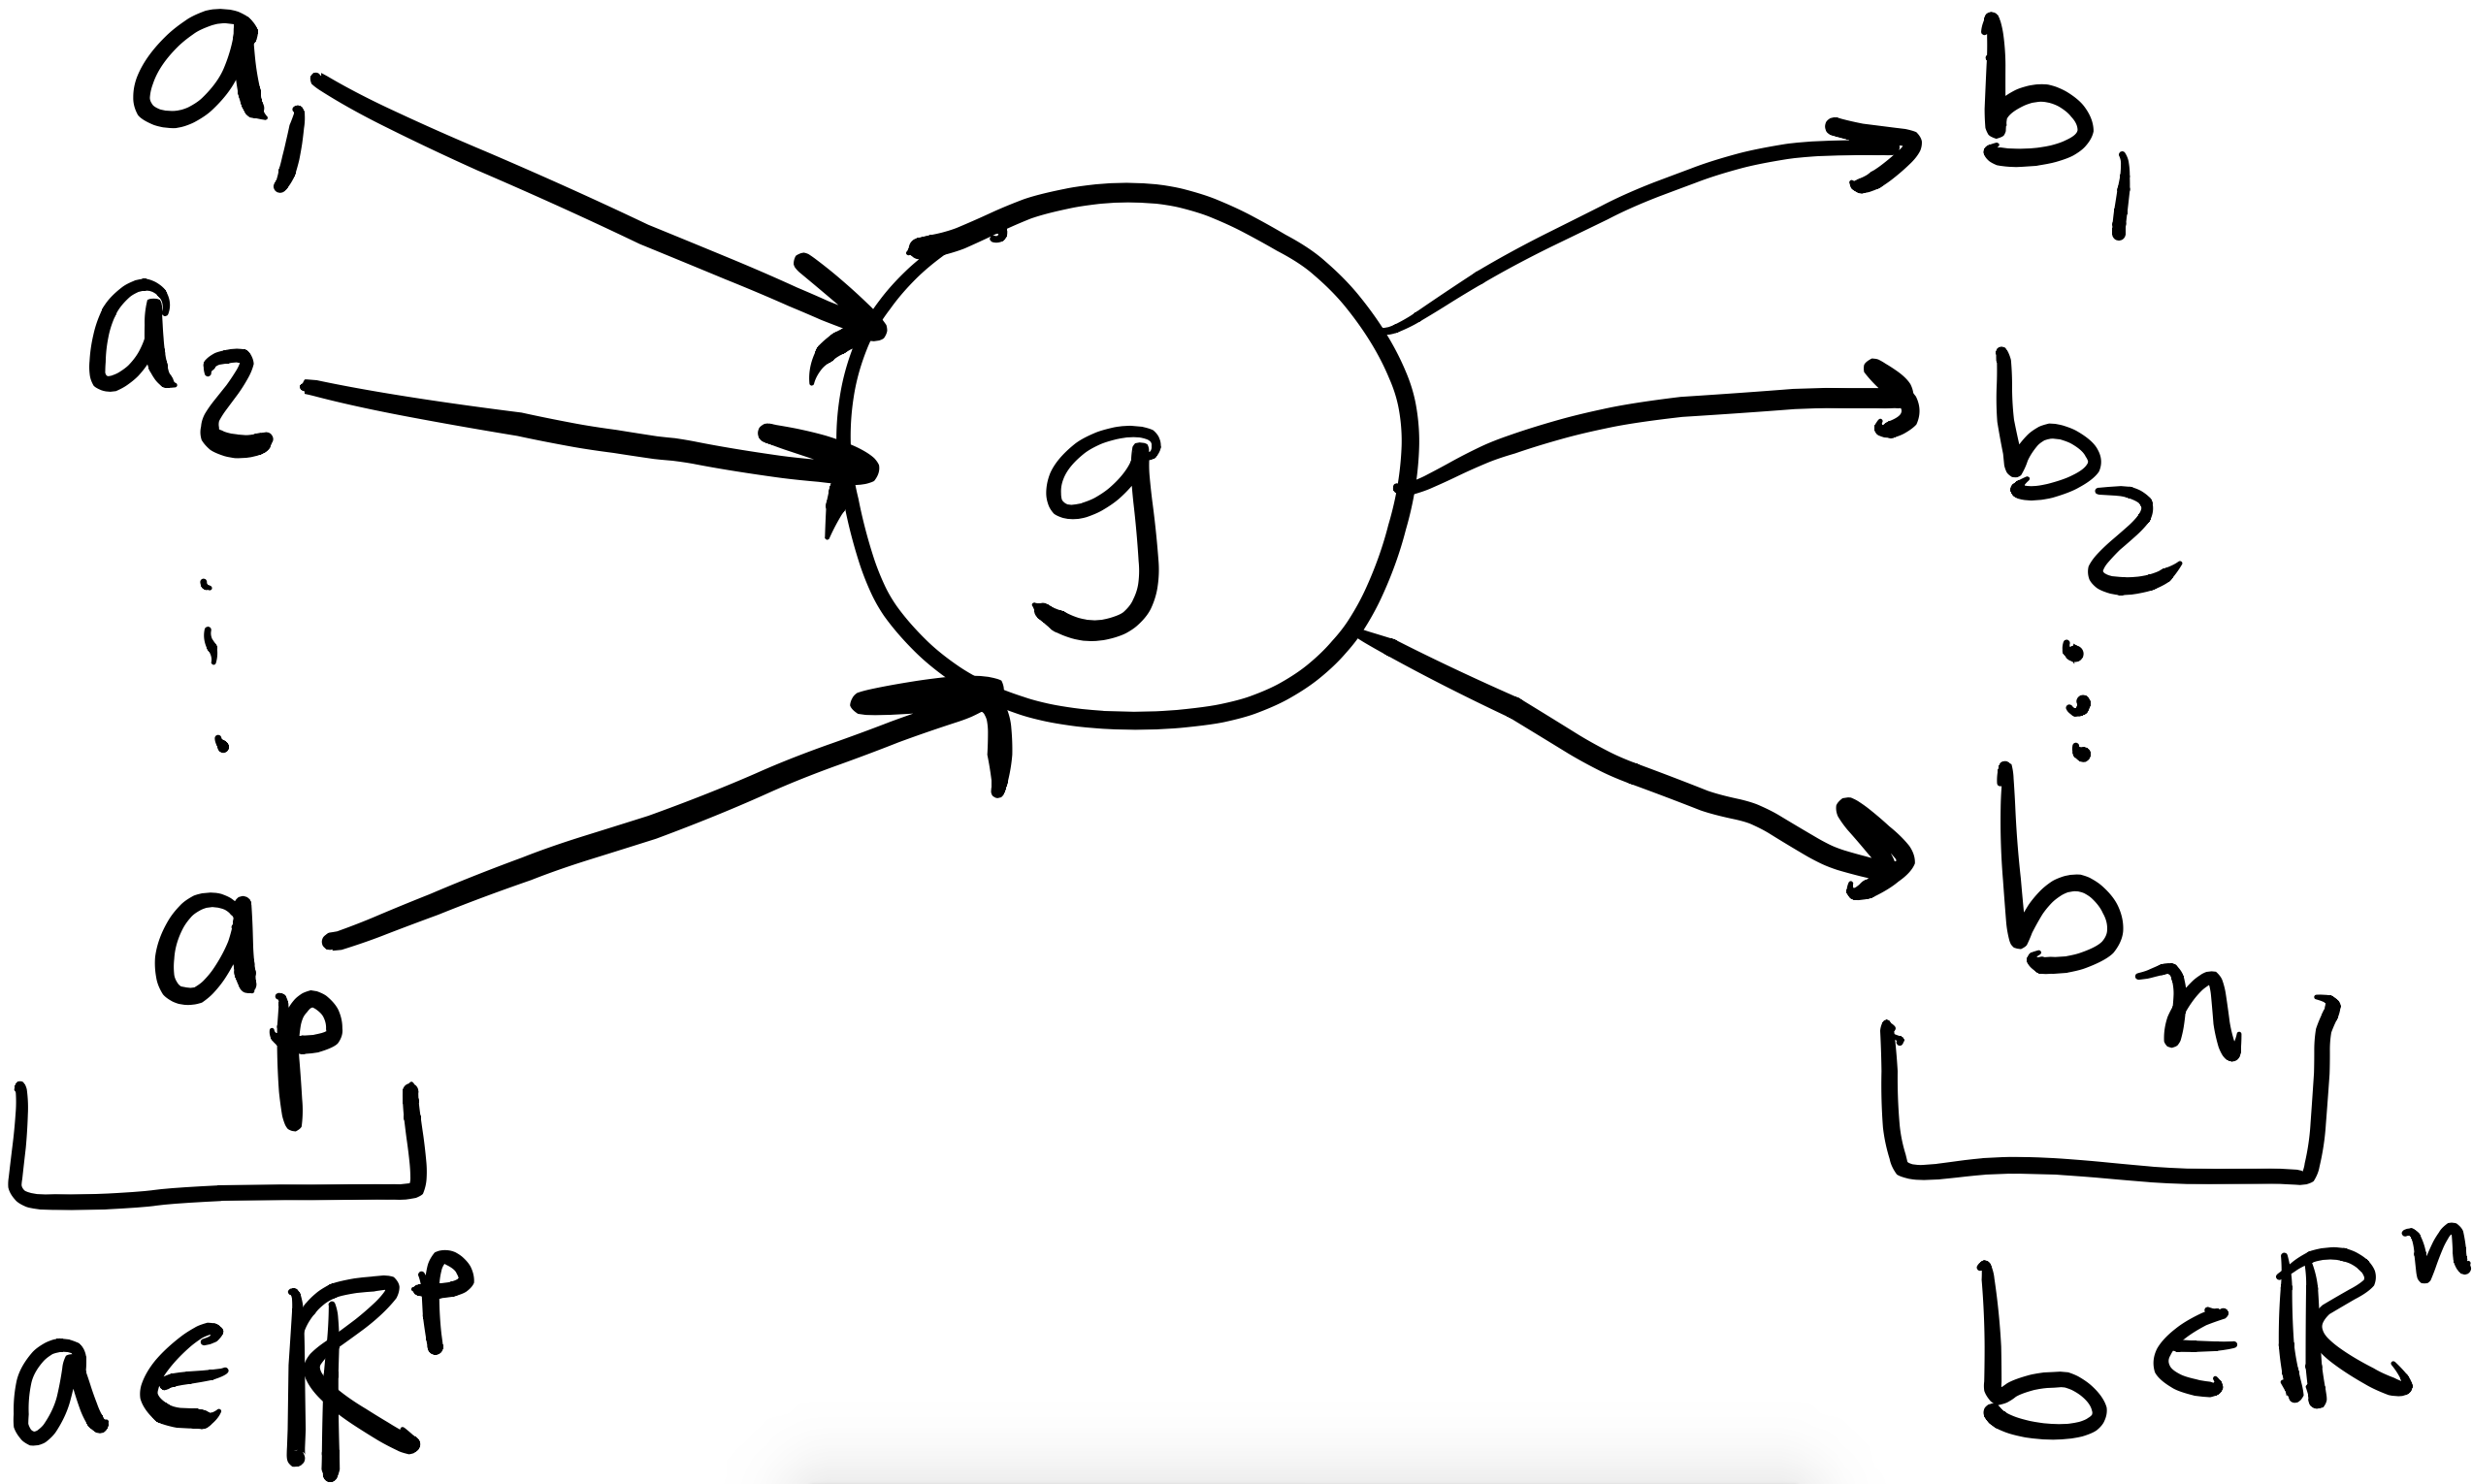
\includegraphics[scale=0.05]{figures/one-fn-comp-graph-partials}
\end{columns}

    \pdfnote{
CG is a useful abstraction for gradient computation on neural networks and implement neural network softwares.
    }
\end{frame}

\begin{frame}
{Compose multiple functions}
Compose two functions $g:\BR^{p}\to\BR^{n}$ and $f:\BR^{n}\to\BR^{m}$.
\begin{figure}
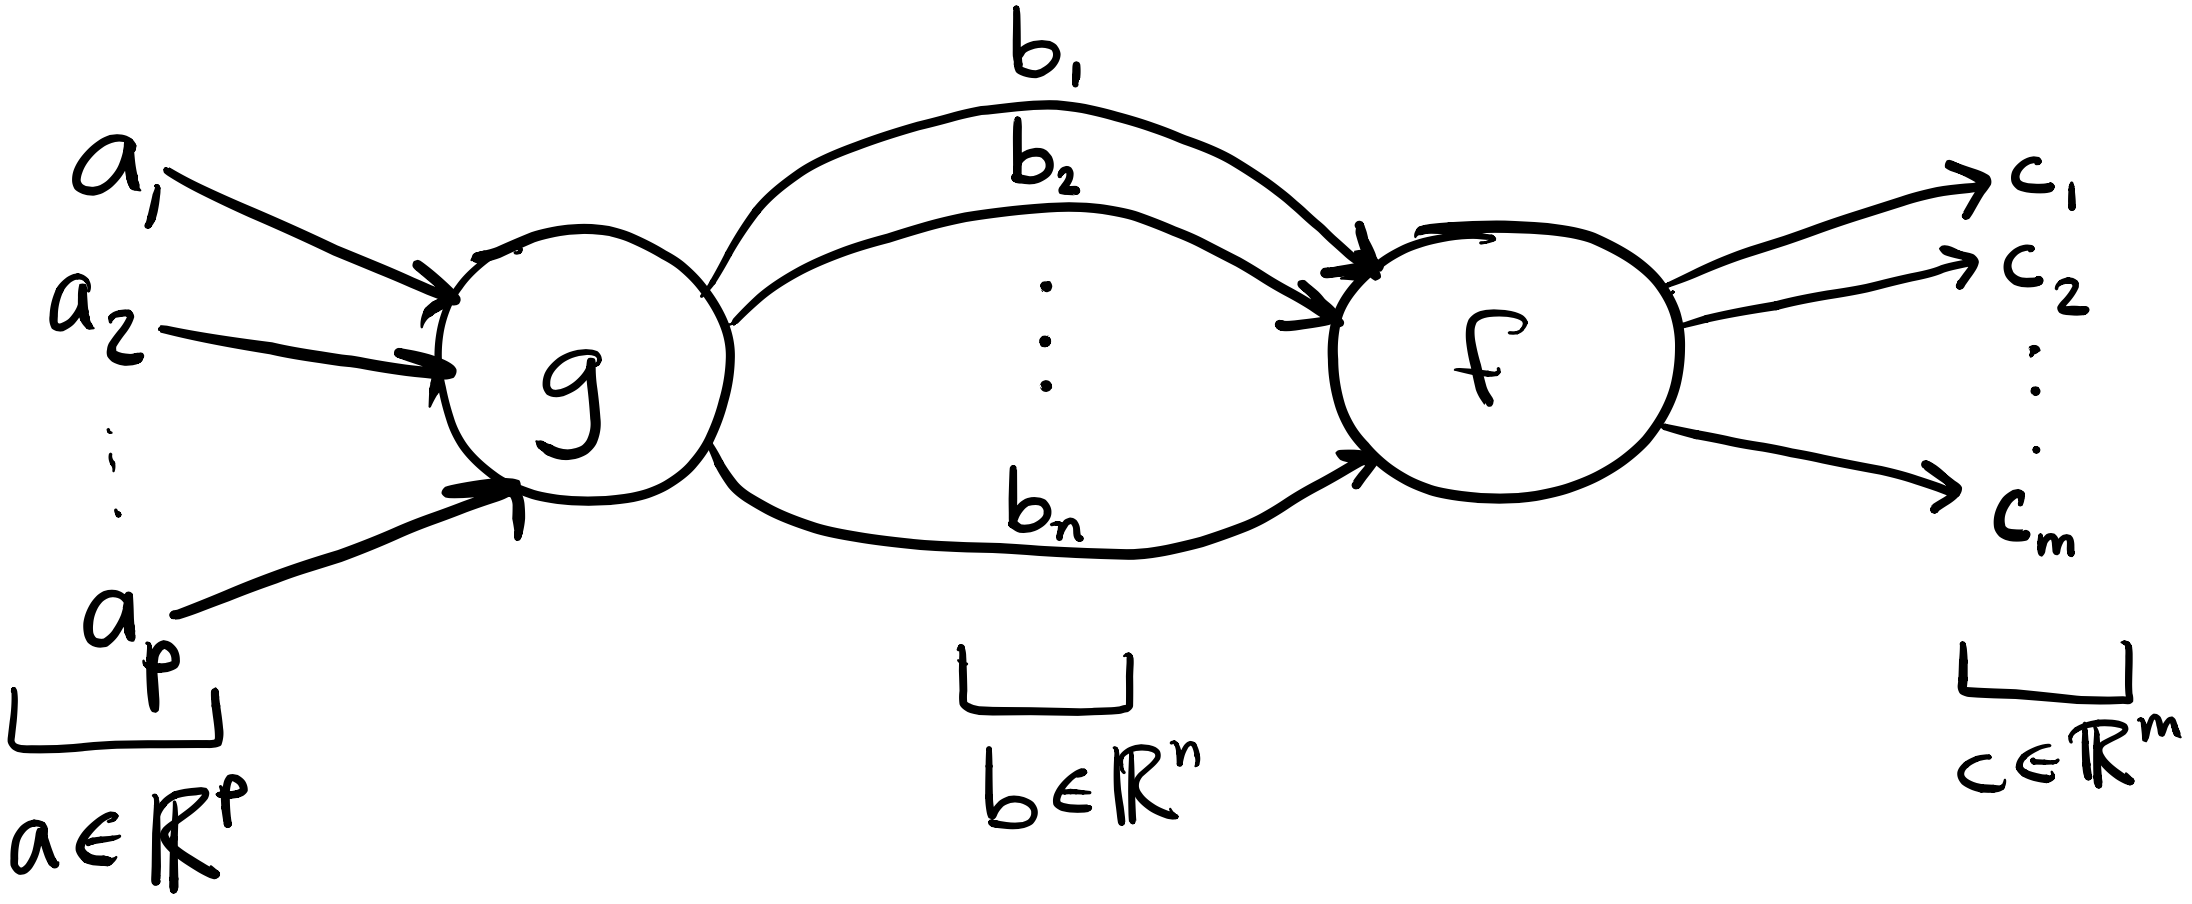
\includegraphics[height=2.5cm]{figures/two-fn-comp-graph-partials}
\end{figure}

\begin{itemize}
    \item $c=f(g(a))$
\item Derivative: How does change in $a_j$ affect $c_i$?
\item Visualize the \textbf{chain rule}:
\begin{itemize}
\item \textcolor{blue}{Sum} changes induced on all paths from $a_j$ to $c_i$.
\item Changes on one path is the {\color{red}product} of changes on each edge.
\[
\frac{\partial c_{i}}{\partial a_{j}}={\color{blue}\sum_{k=1}^{n}}
{\color{red} \frac{\partial c_{i}}{\partial b_{k}}\frac{\partial b_{k}}{\partial a_{j}}} .
\]
\end{itemize} 
\end{itemize}
\end{frame}

\begin{frame}
    {Computation graph example}
    \begin{columns}
\column{.45\textwidth}
        \onslide<1->{
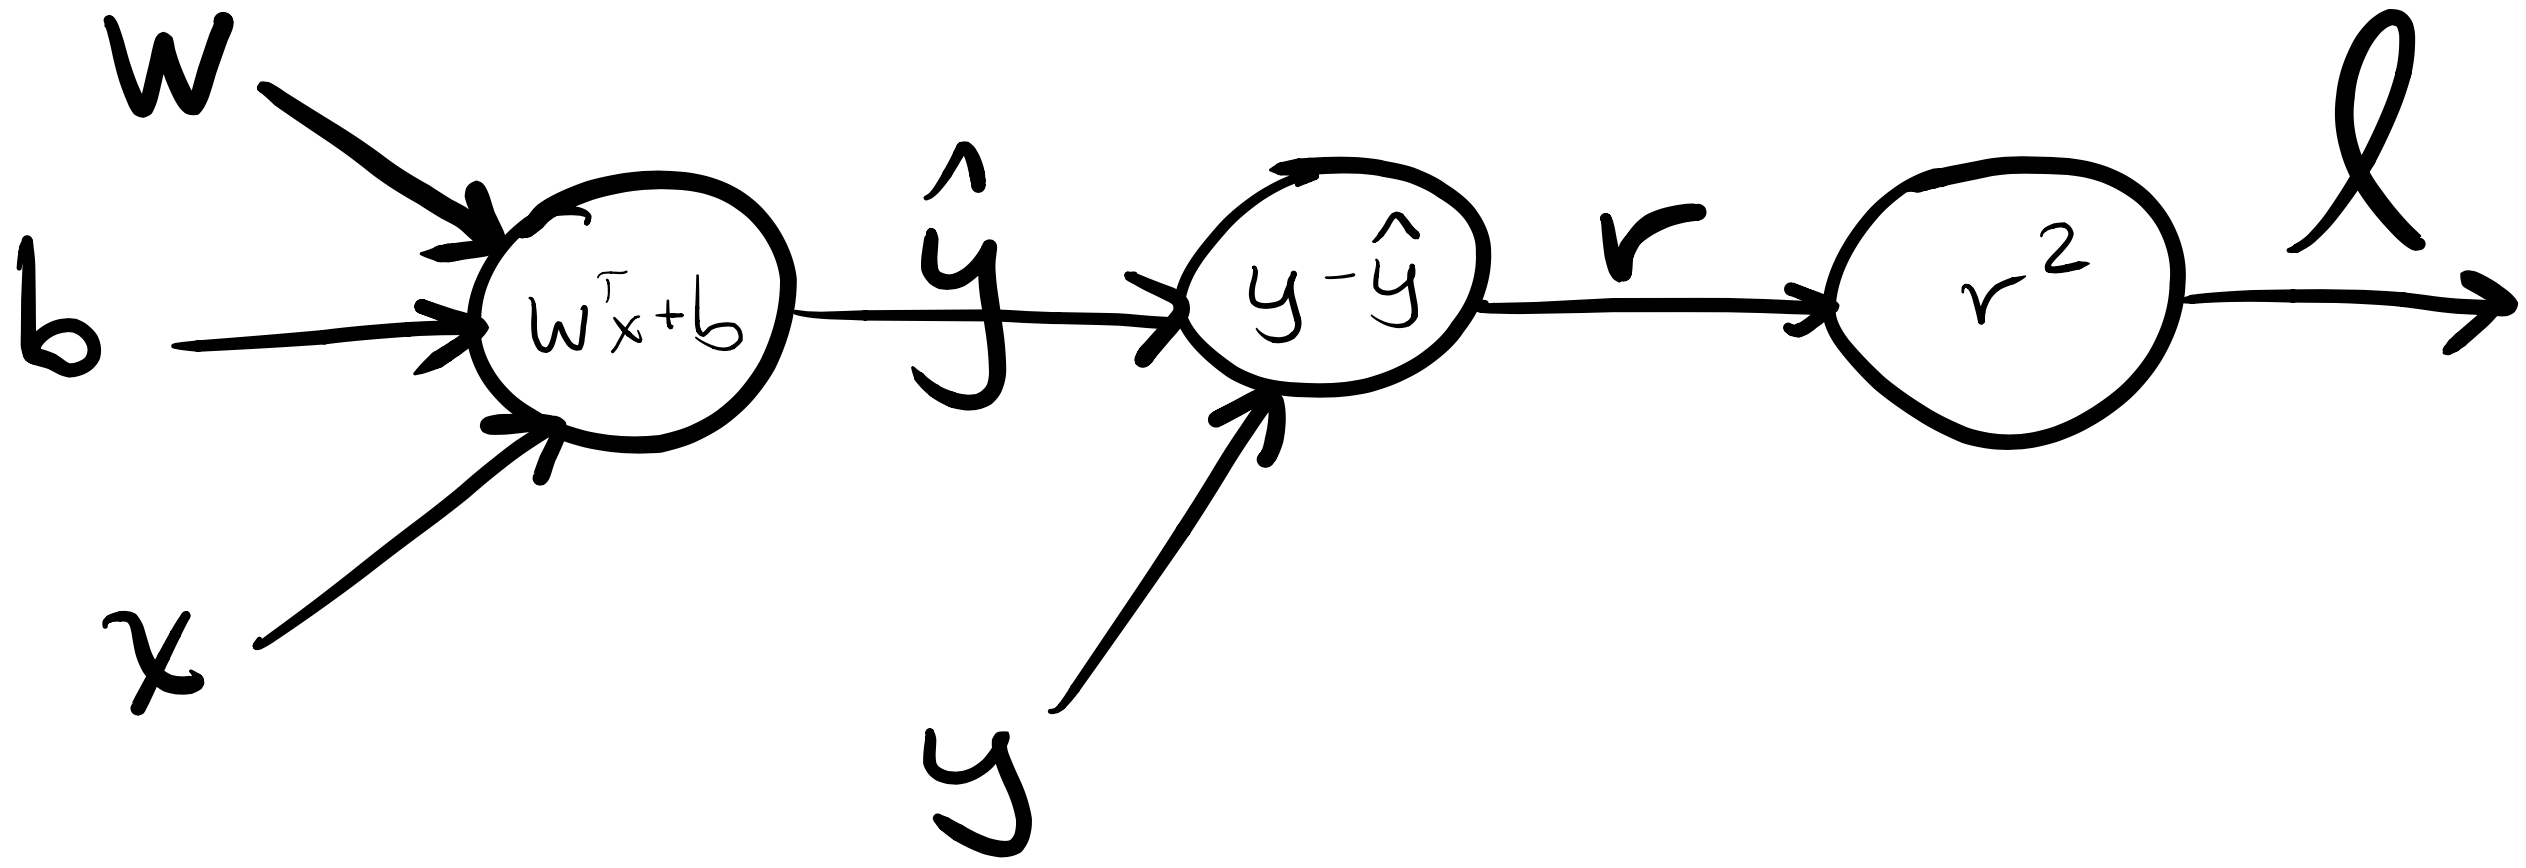
\includegraphics[width=1\textwidth]{figures/linear-sqr-loss-comp-graph}
        \pdfnote{What's the function?}
    }


\column{.45\textwidth}

\begin{eqnarray*}
    \onslide<3->{
\frac{\partial\ell}{\partial r} & = & 2r\\
\frac{\partial\ell}{\partial\hat{y}} & = & \frac{\partial\ell}{\partial r}\frac{\partial r}{\partial\hat{y}}=\left(2r\right)(-1)=-2r\\
    }
    \onslide<2->{
\frac{\partial\ell}{\partial b} & = & \frac{\partial\ell}{\partial\hat{y}}\frac{\partial\hat{y}}{\partial b}=\left(-2r\right)(1)=-2r\\
\frac{\partial\ell}{\partial w_{j}} & = & \frac{\partial\ell}{\partial\hat{y}}\frac{\partial\hat{y}}{\partial w_{j}}=\left(-2r\right)x_{j}=-2rx_{j}
    }
\end{eqnarray*}
\end{columns}
    \pdfnote{Our goal is to compute del l over del w and b which are our params. We can directly compute them or follow this order.}
    \pdfnote{However, note that there is repeated computation}

    Example from David Rosenberg.
\end{frame}

\begin{frame}
    {Backpropogation}
    Backpropogation = chain rule + dynamic programming on a computation graph

    Forward pass
\begin{itemize}
\item \textbf{Topological order}: every node appears before its children
\item For each node, compute the output given the input (from its parents).
\end{itemize}
\begin{center}
\begin{tikzpicture}[shorten >=1pt]
      	\tikzstyle{unit}=[draw,shape=circle,minimum size =1cm]

		\node (start) at (0,1){$\ldots$};
       	\node[unit](i) at (3,1){$f_i$};
        	\node[unit](j) at (6,1){$f_j$};
        	\node (end) at (9,1){$\ldots$};

        	\draw[->] (i) -- (j);
        	\draw[->] (start) -- (i);
        	\draw[->] (j) -- (end);
		
		\begin{scope}[transform canvas={yshift=-.7em}]
		\draw [->, Green, line width=0.05cm, shorten <=1mm, shorten >=1mm] (start) -- node {} (i);
  		\draw [->, Green, line width=0.05cm, shorten <=1mm, shorten >=1mm] (i) -- node {} (j);
  		\draw [->, Green, line width=0.05cm, shorten <=1mm, shorten >=1mm] (j) -- node {} (end);
		\end{scope}
		
		\begin{scope}[transform canvas={yshift=-1.4em}]
		\node (i-in) [right=0.2cm of start] {$a$};
		\node (j-in) [right=0.2cm of i] {$b=f_i(a)$};
		\node (j-out) [right=0.2cm of j] {$c=f_j(b)$};
		\end{scope}
\end{tikzpicture}
\end{center}
    \vspace{3em}
\end{frame}

\begin{frame}
    {Backpropogation}
    Backward pass
\begin{itemize}
\item \textbf{Reverse topological order}: every node appear after its children
\item For each node, compute the partial derivative of its output w.r.t. its input, multiplied by the partial derivative from its children (chain rule).
\end{itemize}
\begin{center}
\begin{tikzpicture}[shorten >=1pt]
      	\tikzstyle{unit}=[draw,shape=circle,minimum size =1cm]

		\node (start) at (0,1){$\ldots$};
       	\node[unit](i) at (3,1){$f_i$};
        	\node[unit](j) at (6,1){$f_j$};
        	\node (end) at (9,1){$\ldots$};

        	\draw[->] (i) -- (j);
        	\draw[->] (start) -- (i);
        	\draw[->] (j) -- (end);
		
		\begin{scope}[transform canvas={yshift=-.7em}]
		\draw [->, Green, line width=0.05cm, shorten <=1mm, shorten >=1mm] (start) -- node {} (i);
  		\draw [->, Green, line width=0.05cm, shorten <=1mm, shorten >=1mm] (i) -- node {} (j);
  		\draw [->, Green, line width=0.05cm, shorten <=1mm, shorten >=1mm] (j) -- node {} (end);
		\end{scope}
		
		\begin{scope}[transform canvas={yshift=-1.4em}]
		\node (i-in) [right=0.2cm of start] {$a$};
		\node (j-in) [right=0.2cm of i] {$b=f_i(a)$};
		\node (j-out) [right=0.2cm of j] {$c=f_j(b)$};
		\end{scope}
		
		\begin{scope}[transform canvas={yshift=-2.5em}]
		\draw [<-, red, line width=0.05cm, shorten <=1mm, shorten >=1mm] (start) -- node {} (i);
  		\draw [<-, red, line width=0.05cm, shorten <=1mm, shorten >=1mm] (i) -- node {} (j);
%  		\draw [<-, red, line width=0.05cm, shorten <=1mm, shorten >=1mm] (j) -- node {} (end);
		\end{scope}
		
		\begin{scope}[transform canvas={yshift=-3.4em}]
		\node (i-out) [left=0.2cm of i] {$g_i=g_j \cdot \frac{\partial b}{\partial a} = \frac{\partial J}{\partial a}$};
		\node (j-out) [left=0.2cm of j] {$g_j=\frac{\partial J}{\partial b}$};
		\end{scope}
\end{tikzpicture}
\end{center}
    \pdfnote{Each node takes the gradient passed from its child. If there are multiple children, then the gradients are added together. Then it computes the dot product of the gradient from its children and its local gradient. And pass the result to its parents.}
\end{frame}

\begin{frame}
    {Summary}
    Neural networks\\
    \begin{itemize}
        \item Automatically learn the features
        \item Optimize by SGD (implemented by back-propogation)
        \item Non-convex, may not reach a global minimum
    \end{itemize}

    Feed-forward neural language models\\
    \begin{itemize}
        \item Use fixed-size context (similar to n-gram models)
        \item Represent context by feed-forward neural networks
    \end{itemize}
\end{frame}

\section{Recurrent Neural Networks}

\begin{frame}
    {Recurrent neural networks}
    How much context is needed?\\
    ... I went $\rule{1cm}{0.15mm}$ $\rule{1cm}{0.15mm}$
    \pdfnote{"to" doesn't need much context, but the next word does}

    Idea: combine new context with old context recurrently to handle varying context sizes 
    $$
 h_t = \sigma(\underbrace{W_{hh}h_{t-1}}_{\textstyle\text{previous state}}+
 \underbrace{W_{ih}x_t}_{\textstyle\text{new input}} + b_h)
 \;.
    $$
    \pdfnote{
        RNN is a model for sequence data.
        We add a piece of new information at each time step.
    Specifically, we maintain a representation of the current state, which summarizes the context until the current time step.
    To compute the current state, we take the previous state and combine it with the new input.
    }

    \begin{figure}
        \includegraphics[height=3cm]{figures/rnn}
    \end{figure}
    \pdfnote{
        Here x are word embeddings, so we are omitting the input embedding layer that maps one-hot representation of words to dense word vectors.
    }
    \pdfnote{
        The recurrent unit has two learnable matrices to combine prev state and input.
    }
    \pdfnote{
        The output o is a real vector, and we can take that as a feature vector of each word with the left context,
        which can be then used to predict the next word.
    }
\end{frame}

\begin{frame}
    {Backpropogation through time}
    %Exercise: compute $\frac{\partial h_t}{\partial h_i}$
    $$
 h_t = \sigma(\underbrace{W_{hh}h_{t-1}}_{\text{previous state}}+
 \underbrace{W_{ih}x_t}_{\text{new input}} + b_h)
 \;.
    $$

    \gray{[board]}

    Problem:\\
    \begin{itemize}
        \item Gradient involves repeated multiplication of $W_{hh}$
        \item Gradient will vanish / explode
    \end{itemize}

    Quick fixes:\\
    \begin{itemize}
        \item Truncate after $k$ steps (i.e. \texttt{detach} in the backward pass)
        \item Gradient clipping
    \end{itemize}
\end{frame}

\begin{frame}
    {Long-short term memory (LSTM)}
    %\emph{Key idea}: have a separate mechanism to decide when to ``memorize'' or ``forget'' a state

    \begin{itemize}
        \item \blue{Memory cell}: decide when to ``memorize'' or ``forget'' a state
            \begin{align*}
                c_t &= \underbrace{i_t \odot \tilde{c}_t}_{\textstyle\text{update with new memory}} +
     \underbrace{f_t \odot c_{t-1}}_{\textstyle\text{reset old memory}}\\
                \tilde{c}_t &= \tanh(W_{xc}x_t + W_{hc}h_{t-1} + b_c) \;.
            \end{align*}

            \item Input gate and forget gate
            \begin{align*}
 i_t &= \text{sigmoid}(W_{xi}x_t + W_{hi}h_{t-1} + b_i) \;,\\
 f_t &= \text{sigmoid}(W_{xf}x_t + W_{hf}h_{t-1} + b_f) \;.
            \end{align*}

            \item Hidden state
            \begin{align*}
 h_t &= o_t \odot c_t \;\text{, where} \\
 o_t &= \text{sigmoid}(W_{xo}x_t + W_{ho}h_{t-1} + b_o) \;.
            \end{align*}
    \end{itemize}
    Gating allows the network to learn to control how much gradient should vanish.
    \pdfnote{
        How does it fix the gradient vanishing/exploding problem?
        With RNN our problem is that we end with repeated multiplication of the same matrix.
        Try compute del c(t) over del c(t-1).
        It still involves repeated multiplication of certain quantity, but it will depend on learned values that are different at each time step, specifically the input and forget gates.
        So the network can decide when to reset the gradient or to increase the gradient signal depending on whether there is long-range dependencies in the data.
    }
\end{frame}

\section{Evaluation}
\begin{frame}
    {Perplexity}
    What is the loss function for learning language models?
    \pause

    Held-out likelihood on test data $D$:
    $$
    \ell({D}) = \sum_{i=1}^{|D|} \log p_\theta(x_i\mid x_{1:i-1}) \;,
    $$
    \pdfnote{In practice, no sentence segmentation, a sequence of words, average likelihood of each word}
    \pause

    \textbf{Perplexity}:
    $$
 \text{PPL}(D) = 2^{-\frac{\ell(D)}{|D|}} \;.
 $$
    \begin{itemize}
        \item Base of log and exponentiation should match
        \item Exponent is cross entropy: $H(p_{data}, p_\theta) = -\BE_{x\sim p}\log p_\theta(x)$.
            \pdfnote{Entropy is the number of bits needed to encode an event from a certain distribution.}
            \pdfnote{Cross-entropy is the number of bits needed to encode an event from a certain distribution (here p data) when your coding scheme is optimized for another distribution (here p theta).}
        \item Interpretation: a model of perplexity $k$ predicts the next word by throwing a fair $k$-sided die.
            \pdfnote{2 to the number of bits: total number of outcomes}
            \pdfnote{Sanity check: if PPL is larger than vocab size, something must be wrong.}
    \end{itemize}
\end{frame}

\end{document}
